\documentclass[12pt]{article}

\usepackage{sbc-template} 
\usepackage{graphicx,url}
\usepackage{url}
 \usepackage[spanish]{babel}
\usepackage[utf8]{inputenc} 
\usepackage[T1]{fontenc}
\usepackage[normalem]{ulem}
\usepackage[hidelinks]{hyperref}
\usepackage{rotating}

\usepackage[square,authoryear]{natbib}
\usepackage{amssymb} 
\usepackage{mathalfa} 
\usepackage{algorithm} 
\usepackage{algpseudocode} 
\usepackage[table]{xcolor}
\usepackage{array}
\usepackage{titlesec}
\usepackage{mdframed}
\usepackage{listings}
\usepackage{subfigure} 
\usepackage{amsmath} 
\usepackage{booktabs}

%\usepackage{caption}
%\usepackage{subcaption}

\urlstyle{same}

\newcolumntype{L}[1]{>{\raggedright\let\newline\\\arraybackslash\hspace{0pt}}m{#1}}
\newcolumntype{C}[1]{>{\centering\let\newline\\\arraybackslash\hspace{0pt}}m{#1}}
\newcolumntype{R}[1]{>{\raggedleft\let\newline\\\arraybackslash\hspace{0pt}}m{#1}}

\newcommand\Tstrut{\rule{0pt}{2.6ex}} 
\newcommand\Bstrut{\rule[-0.9ex]{0pt}{0pt}} 
\newcommand{\scell}[2][c]{\begin{tabular}[#1]{@{}c@{}}#2\end{tabular}}

\usepackage[nolist,nohyperlinks]{acronym}

\title{Aplicación de técnicas de Inteligencia Artificial 
al sector de producción de energías renovables}

%\author{Nome do Autor\inst{1}}


% \address{Instituto Federal de Educação, Ciência e Tecnologia de Rondônia - IFRO
% 	\email{email@aluno.ifro.edu.br}
% }

\begin{document} 
	
	\maketitle
	
	\section{Introducción}
	\label{sec:motivacion}
	
En la actualidad, los países desarrollados están impulsando políticas que promueven el uso de energías renovables, tal como se explica en los "White Papers" de la Unión Europea \citep{Garcia}. Entre estas fuentes de energía, la eólica se destaca por su importancia, y se estima que para el año 2030 representará el 33$\%$  del consumo de electricidad en la UE, llegando incluso al 50$\%$  en un largo plazo (2030-2050) \citep{Amanatidis,Mitchell}. Además, en los últimos años, una parte importante de los sistemas de conversión de energía han estado utilizando la energía de las olas del océano \citep{Mahsa}. Cada vez más, la toma de decisiones en estos procesos de generación de energía se apoyan en algoritmos de Inteligencia Artificial (IA).

De acuerdo con Scopus, entre 1970 y 2019 se realizaron 15,368 publicaciones sobre técnicas de IA aplicadas a la producción de energía \citep{Garcia}. En el ámbito de las energías renovables, en particular de la energía generada por turbinas eólicas marinas flotantes (FOWTS), estas técnicas se emplean principalmente en sistemas de monitoreo, gestión y mantenimiento. Una tarea fundamental en el diseño de FOWTS es verificar su viabilidad y comportamiento, y para ello se realizan predicciones utilizando algoritmos de IA \citep{Chen}. La optimización es una de las aplicaciones más comunes para la mayoría de las técnicas de IA, donde se traducen las variables ambientales a términos económicos para facilitar la toma de decisiones y la planificación. Otra aplicación importante es la detección de fallos mediante el análisis de señales y el reconocimiento de patrones. Por ejemplo, uno de los principales desafíos al elegir los sitios adecuados para la construcción de estos dispositivos es predecir cuánta energía se producirá teniendo en cuenta las condiciones climáticas del lugar. Los algoritmos de IA permiten realizar estas predicciones y seleccionar el mejor tipo de dispositivos (turbinas o conversores de olas) para cada emplazamiento \citep{Mahsa}.

Las técnicas de IA más utilizadas son los algoritmos de redes neuronales (NNs), seguidos por los algoritmos genéticos (GA) y la lógica difusa. Las NNs son los modelos más versátiles y se aplican principalmente para la detección de fallos, problemas de optimización, modelización y predicciones, y se combinan con técnicas de big data, análisis de componentes principales PCA y métodos estadísticos. Por otro lado, los algoritmos GA se centran más en resolver problemas de optimización, toma de decisiones y planificación, y otros algoritmos utilizados para estas tareas consideran enjambres de partículas. Los algoritmos de lógica difusa se utilizan principalmente para la toma de decisiones y la mitigación de riesgos, y suelen combinarse con NNs. También se utilizan métodos estadísticos, como Monte Carlo, para el mantenimiento y las predicciones de fallos, para lo cual se utilizan cantidades considerables de datos \citep{Garcia}.

Por ejemplo, \citet{Mahsa, Chen,Zheng} entre otros emplean redes neuronales para predecir la potencia generada por sistemas híbridos que utilizan turbinas eólicas y la energía de olas. Mientras que \citep{yeter} han utilizado estas técnicas para la extensión de la vida útil de las estructuras de las turbinas eólicas marinas flotantes \citep{yeter} y \citet{Xie} aplican DRL para encontrar la mejor estrategia para disipar la energía del oleaje en rompeolas. 
Por otro lado, \citet{Li} utilizan redes neuronales para realizar predicciones en tiempo real de la energía generada por el oleaje mientras que \citet{Li2} de manera similar predicen la velocidad del viento en la costa y \citep{Manuel} estudian el rendimiento de diferentes modelos de ML para la predicción de la precipitación.

En resumen, las técnicas de aprendizaje automático (ML) y Aprendizaje profundo (DL) se han utilizado con éxito en diferentes procesos de generación de energía que utilizan el viento y el oleaje marino. Estas técnicas han permitido mejorar la precisión en la predicción de la potencia generada, simular la dinámica de los dispositivos, y tomar decisiones a tiempo real a partir de datos a gran escala. Se espera que estos avances sigan impulsando el desarrollo de las energías renovables en un futuro cercano.

En las secciones 2, 3  del presente estudio, se examinan dos artículos (\cite{Manuel,Li2}) que emplean modelos de aprendizaje automático para predecir variables climáticas como la precipitación y  la velocidad del viento a diferentes escalas horarios. Y en la sección 4, un artículo (\cite{Mahsa}) en donde se aplican métodos similares para predecir la potencia generada por sistemas híbridos de energía que aprovechan tanto la fuerza de las olas como del viento. Estos análisis son fundamentales para seleccionar la ubicación y el tipo de dispositivo más adecuado en función de las condiciones climáticas de la región de interés.

\section{IA aplicada a la predicción de la precipitación}

Para determinar las condiciones óptimas en la elección de sitios en donde construir dispositivos de generación de energía renovable, es esencial realizar un análisis climatológico que incluya información in situ sobre la altura del oleaje, velocidad del viento en la costa, etc \citep{ Nkiaka, Hasan, Wang,Li,Li2}. Sin embargo, esta información no siempre se encuentra disponible en ciertas áreas del mundo y para muchos períodos temporales \citep{Buytaert}, por lo que se necesitan métodos para completar estos "huecos". Una solución es aplicar técnicas de ML, la principal ventaja de utilizar estas técnicas es que normalmente no se requiere hacer suposiciones sobre la distribución de errores ni conocer de antemano la forma de las relaciones entre los predictores y las variables a predecir \citep{Manuel}.

Por ejemplo, en un artículo reciente, \citet{Manuel} realizaron un estudio comparativo de la capacidad de varios modelos de ML (ver Tabla \ref{tabla0}) para predecir la intensidad (problema de regresión) y cantidad (problema de clasificación) de precipitación en diferentes zonas de Tenerife. Para ello, utilizaron como variables predictoras la elevación, el porcentaje de huecos presentes en las series, la precipitación anual promedio, la ubicación en la isla (norte o sur) y la estacionalidad de las series temporales.

\begin{table}
\centering
% \begin{turn}{90}
\begin{tabular}{|p{2.0cm}|p{14.0cm}| }
\hline
    \textbf{GLM-L:}& Regresión lineal clásica pero asumiendo\newline  una relación logarítmica entre el predictor y el predictando.\\
    &\\
    \textbf{GLM-G:}& Regresión lineal clásica pero asumiendo que los errores siguen una distribución gamma. \\
    &\\
    \textbf{Random Forest (RF):} & Es un método de ML que durante el entrenamiento construye una multitud de árboles de decisión  y predice la moda de las clases (clasificación) o la media de las predicciones (regresión) de los árboles individuales. Hiperparámetros: $N_{est}$: número total de árboles, y $min_{samp-leaf}$: número mínimo de muestras requeridas por nodo hoja, sobre el cual se calcula la moda o la media. \\
    &\\
    \textbf{K-Nearest Neighbors (k-NN)}  &se calcula la moda ponderada (clasificación) o la media ponderada (regresión) de los k puntos más cercanos al que se está prediciendo. Hiperparámetros: $n_{neigh}$: número de vecinos utilizados en la predicción, y $pesos$: función de peso utilizada en la predicción. $Uniforme$ significa que todos los puntos en el vecindario tienen el mismo peso, mientras que $distancia$ significa que los puntos están ponderados por el inverso de su distancia.\\
    &\\
    \textbf{Redes Neuronales (NN)}: &método de ML que aprende relaciones entre una serie de características de entrada (capa de entrada) y una salida (capa de salida) a través de combinaciones lineales y transformaciones no lineales de las entradas recibidas por cada neurona en la red (capa oculta). Hiperparámetros: $Hidden_{layer-sizes}$: número de neuronas y capas utilizadas, $activación$: función no lineal que cada neurona utiliza para transformar la combinación lineal de entradas, y $alpha$: controla la fuerza de la regularización penalizando los pesos con magnitudes grandes.\\
    &\\
    \textbf{Support Vector Machines (SVM)}: & realiza tareas de clasificación y regresión mediante la búsqueda de los hiperplanos que maximizan los márgenes, es decir, la brecha mínima que separa las muestras que pertenecen a diferentes grupos. Los valores más cercanos al margen de clasificación se conocen como $vectores~de~soporte$. Se utilizan kernels de función de base radial (RBF) para asegurar que la separación sea posible en espacios no lineales. Hiperparámetros: $\gamma$: radio del área de influencia de los vectores de soporte, $C$: define un margen de tolerancia donde no se penaliza los errores. \\
    &\\
    \textbf {Weather Typing (WT) o k-Means}:  & es un método que divide el espacio de entrada en regiones y utiliza la moda o la media de la región en la que se encuentra el punto candidato para resolver el problema de clasificación o regresión. En esta aplicación específica, los tipos de clima se calculan utilizando el algoritmo k-Means convirtiendo los tipos de clima en patrones atmosféricos sinópticos representativos. \\    
\hline
\end{tabular}
% \end{turn}
\caption{Descripción de los modelos.}
 \label{tabla0}
\end{table}

Para evaluar el rendimiento de los modelos, se utilizaron diferentes métricas: el f-score para los problemas de clasificación y la suma de los errores cuadráticos para los modelos de regresión. Los datos se separaron en conjuntos de entrenamiento y prueba, en una proporción de 80$\%$-20$\%$, respectivamente. Además, se realizó una búsqueda de hiperparámetros (ver tabla \ref{tabla}) en el conjunto de entrenamiento y se estandarizó y transformó el espacio predictor mediante un análisis de componentes principales (PCA). Esto se hizo para eliminar la correlación espacial entre las variables de diferentes ubicaciones que puede distorsionar los resultados, además diferentes estudios han concluido que, en general, las PCAs son mejores predictores que las variables individuales, probablemente porque agregan información de todo el espacio predictor \citep{Gutiérrez, Preisendorfer, San-Martin}.


\begin{figure}[h!]
\centering
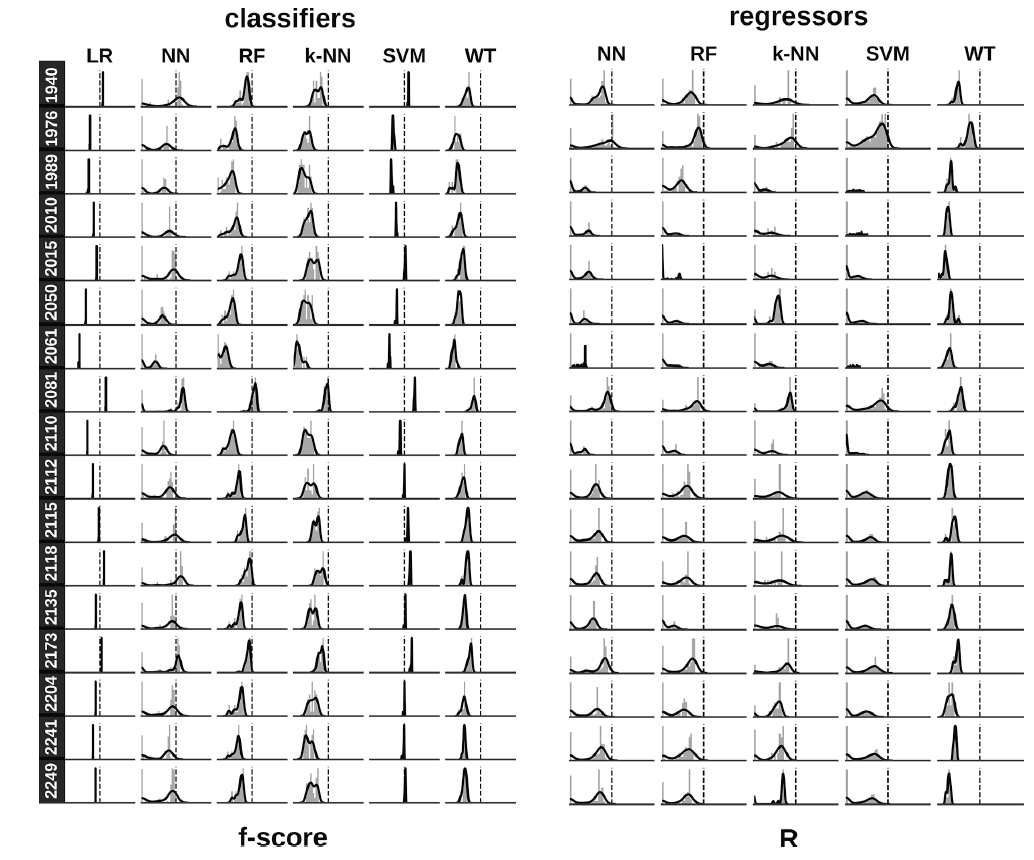
\includegraphics[height=5.5in]{figures/Manu_res0.PNG}
\caption{Figura 4 de \citet{Manuel}: Distribuciones para los valores del f-score en el caso de problemas de clasificación (columna izquierda), y el error en el caso de problemas de regresión (columna derecha).}
\label{Manu_res0}
\end{figure}

Durante el proceso de "\textit{cross validation}" se han probado varios sets de hiperparámetros para encontrar los valores óptimos. En el panel izquierdo de la figura \ref{Manu_res0} se muestra como se distribuyen los valores del f-score en el caso de los modelos utilizados para clasificación, y en la columna derecha la distribución del error en el caso de problemas de regresión. Se puede observar que los modelos GLM , RF y WT no dependen fuertemente de los valores de los hiperparámetros utilizados, de hecho los primeros dos muestran distribuciones que son prácticamente deltas de Dirac. Esto indica que los resultados de estos modelos dependen de las características de las series a predecir y no pueden ser fácilmente ajustados variando los hiperparámetros. Por otro lado, las NNs muestran distribuciones ampliamente extendidas lo que indica una gran sensibilidad a los hiperparámetros. Los métodos de RF y KNN se encuentran en un espectro intermedio, su rendimiento es sensible a los hiperparámetros, pero sus distribuciones son más estrechas que las de las NNs.

Los resultados (Fig. \ref{Manu_res0}) del estudio indican que las NNs son los modelos que presentan un mejor rendimiento en términos de las métricas consideradas. Se realizaron múltiples pruebas de hipótesis para verificar si la mejora en comparación con otros modelos es significativa y se encontró que las NNs funcionan significativamente mejor que otros modelos para predecir tanto la ocurrencia como la intensidad de lluvia. En segundo lugar, los modelos de regresión logística (LR) y SVM presentan mejoras significativas en comparación con los modelos de RF, K-NN y WT. Un hallazgo interesante es que los modelos NN, LR y SVM son los únicos capaces de simular meses inusualmente húmedos (con más de 20 días húmedos).


\section{IA aplicada a la predicción de la velocidad del viento.}

Como se ha mencionado anteriormente, la predicción de la velocidad del viento es crucial para estimar la energía que se puede generar en las FOWTS.
\citet{Li2} presentan un estudio comparativo utilizando diferentes modelos de redes neuronales para la predicción de la velocidad del viento en la costa 
a corto plazo (1 hr) en dos locaciones diferentes:  Hann y Kulm en Dakota del Norte. En ambos sitios se ha medido la velocidad promedio del viento por horas y se ha almacenado en series que abarcan un año. 

Los modelos considerados son el modelo BF, modelo RBF, y modelo ADALINE. El modelo BF (Figura \ref{BP}) es un modelo estándar de \textit{"Forward-Back propagation"}, con funciones de activación sigmoideas en la capa oculta y función lineal en la capa de salida. Se consideran los bias $b_{HI}$ y $b_{HO}$ para la capa oculta y la capa de salida, respectivamente. Por otro lado, el modelo RBF (Figura \ref{RBF}) utiliza una superposición de funciones radiales como función de activación en la capa oculta:
\begin{equation}
f(x)=\sum c_i h(||x-x_i||)
\end{equation}
Estas funciones dan lugar a resultados diferentes de cero dentro de una pequeña región en el espacio de inputs definida por la distancia $r=||x-x_i||$, donde $x_i$ satisface la condición $f(x_i)=y_i$, que a su vez determina los valores de $c_i$. 
La estructura del modelo ADALINE se puede ver en la Figura \ref{ADALINE}, en este caso no se plica una función de activación en las capas ocultas, por lo que simplemente se realiza una combinación lineal de los pesos y por lo tanto este modelo solo puede resolver problemas linealmente separables. Sin embargo, el algoritmo de mínimos cuadrados medios o "least mean squared" (LMS) puede minimizar el error cuadrático medio (MSE) y buscar el punto mínimo global en el espacio de los pesos, lo que permite mover las fronteras de decisión tan lejos como sea posible de los patrones de entrenamiento.

\begin{figure}[h!]
\centering
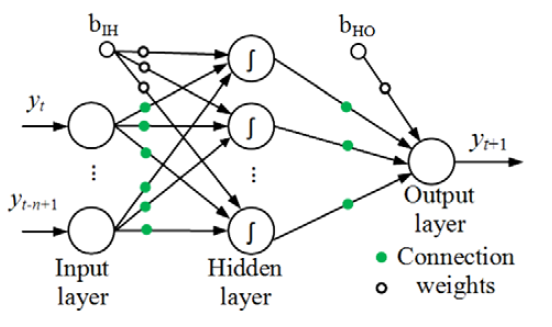
\includegraphics[height=1.5in]{figures/BP.PNG}
\caption{Modelo BP (Figura 1 de \citet{Li2}).}
\label{BP}
\end{figure}

\begin{figure}[h!]
\centering
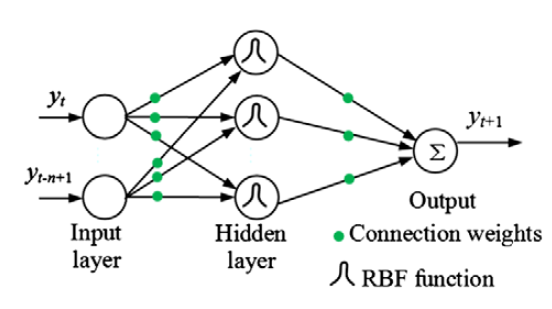
\includegraphics[height=1.5in]{figures/RBF.PNG}
\caption{Modelo RBF (Figura 2 de \citet{Li2}).}
\label{RBF}
\end{figure}

\begin{figure}[h!]
\centering
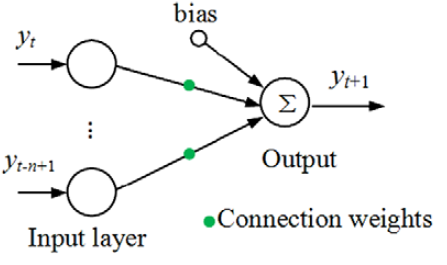
\includegraphics[height=1.3in]{figures/ADALINE.PNG}
\caption{Modelo ADALINE (Figura 3 de \citet{Li2}).}
\label{ADALINE}
\end{figure}

Los inputs para las redes neuronales son las observaciones de la velocidad del viento entre un tiempo $t-n+1$ y $t$, y el output es la predicción para el tiempo $t+1$. Se han considerado tres métricas diferentes para definir la función de pérdida: el error medio absoluto (MAE) el error cuadrático medio (RMSE) y el error de porcentaje absoluto medio (MAPE).
El tamaño del input de las redes neuronales depende entonces del tiempo de retardo (\textit{lag}), es decir, cuántas observaciones previas se encuentran correlacionadas con el valor correspondiente al tiempo $t+1$. Éste se puede estimar mediante herramientas estadísticas (función de auto-correlación y función de auto-correlación parcial). Para los modelos considerados, el \textit{lag} varía entre 1 y 8. 
Las observaciones utilizadas para predecir cada tiempo se pre-procesan y se ordenan en un vector, posteriormente el data set pre-procesado se divide en tres conjuntos: \textit{train-evaluation-test}. El número óptimo de capas ocultas para los modelos BF y ADALINE es aproximadamente $log(T)$, donde $T$ es el número de vectores de entrenamiento, mientras que el número optimo para el modelo RBF se optimiza iterativamente durante el entrenamiento.

En la figura \ref{Li2_res},  se muestran los resultados obtenidos para los modelos con mayor y menor RSME para los sitios de Hann y Kulm en Dakota del Norte. Observando estas gráficas se puede concluir que la precisión obtenida considerando los diferentes modelos es similar, la diferencia radica mayormente en la eficiencia en la convergencia de los modelos. Por ejemplo, los autores concluyen que las redes RBF son las que convergen más rápido y además son capaces de encontrar más fácilmente el mínimo global, mientras que los modelos BP tienen más riesgo de caer en mínimos locales. Por otro lado, los autores resaltan que la exactitud de las predicciones de los modelos de redes neuronales está influenciada por varios factores, como el tipo de modelo, los inputs y los \textit{"learning rates"} utilizados. Por lo tanto, la elección de un modelo adecuado puede resultar difícil, ya que diferentes métricas pueden dar lugar a diferentes resultados. Para solucionar este problema, diferentes estudios han propuesto investigaciones para desarrollar un índice que combine diferentes métricas para medir la precisión de las predicciones \citep{Tseng,Daga}.

\begin{figure}
    \centering
    \subfigure[]{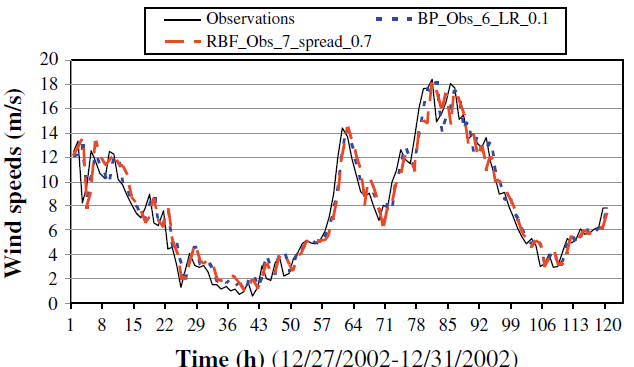
\includegraphics[width=0.8\textwidth]{figures/Li2_1.png}} 
    \subfigure[]{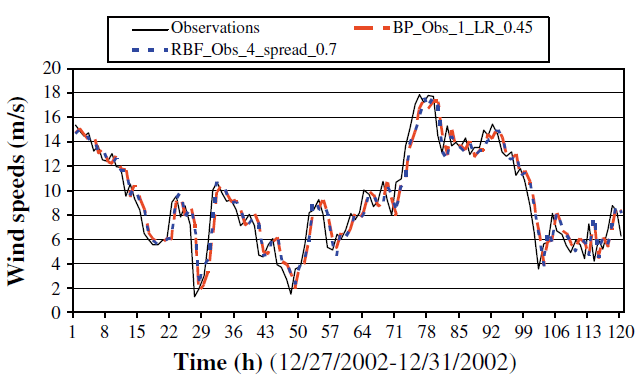
\includegraphics[width=0.8\textwidth]{figures/Li2_3.png}}
    \caption{figuras 7 y 10 de \cite{Li2}. (a)  muestra los resultados para los modelos con mayor y menor RSME obtenidos para el sitio de Hann Dakota del norte. (b)  muestra los mismos resultados pero para el sitio de Kulm, Dakota del Norte.}
    \label{Li2_res}
\end{figure}

En general, en términos de predecir series temporales, se ha descubierto que las redes neuronales funcionan mejor que los modelos persistentes, pero la mejora en la precisión de las predicciones a veces no es significativa \citep{Lei,Sfetsos,Costa}.
Además, se ha observado que los modelos de redes neuronales no son trasladables en el espacio, lo que significa que un modelo que funciona bien en un sitio no necesariamente funciona igual de bien en otro. Para superar este problema de inconsistencia en la selección del modelo, se necesita un método robusto que sea capaz de combinar diferentes modelos de NNs. 
 Por último, los autores destacan  que solo se evaluaron datos de un año  y que sería ideal poseer más datos de entrenamiento de diferentes años para abordar la influencia de la variabilidad inter-anual en el pronóstico de la velocidad del viento. Esta es una limitación de los modelos actuales obtenidos.
 
\section{IA aplicada a la predicción de la generación de energía}
Uno de los mayores desafíos en la selección de sitios adecuados para la construcción de FOWTS  es la capacidad de predecir la cantidad de energía que se producirá en función de las condiciones climáticas del lugar. \citet{Mahsa} han utilizado cuatro algoritmos de ML para predecir la cantidad de energía producida por sistemas híbridos de generación de energía que utilizan turbinas de viento VBT (\textit{Vortex Bladeless Turbine}) y conversores de energía de olas Searasers. 

Para abordar este problema, se ha utilizado como espacio predictor datos de la velocidad del viento y la altura de las olas provenientes de un modelo de cambio climático \citep{He}, y como variables objetivos la fuerza y potencia medidas en algunos emplazamientos. Por otro lado, las bases de datos de entrenamiento se ha enriquecido utilizando simulaciones del software FLOW-3D. Este software utiliza modelos numéricos para simular las interacciones entre los fluidos y las estructuras de los diferentes componentes del dispositivo híbrido, incluyendo la estructura del VBT y el flujo del aire, así como el flujo de las olas y el \textit{Searaser}.
Al entrenar los modelos, se dividieron los datos de entrenamiento en un conjunto de train/test del $90-10 \%$ y se utilizaron cuatro algoritmos de ML:  redes neuronales recurrentes (RNN), redes neuronales recurrentes de memoria a largo plazo (LSTM), Random Forest y SVM con el truco del método de kernel para ampliar el espacio de variables predictoras. Los modelos de RNN y LSTM incluyeron capas convolucionales para capturar patrones espaciales y la dependencia temporal de los datos. 

Los autores concluyeron que los algoritmos RNN y LSTM son los que mejor simulan los valores para la fuerza y la potencia observada/simulada para los dos dispositivos BVT y Searaser (ver Fig. \ref{Mahsa_res3}). Las redes LSTM funcionan mejor que las RNN, mientras que el modelo de Random Forest no funcionó tan bien como se esperaba . 
Por otro lado, los valores máximos y mínimos de la potencia producida pertenecen al Searaser y al VBT, respectivamente. Además, se ha concluído que la fuerza de arrastre en los VBT se puede aproximar con una función cuadrática, mientras que la fuerza total ejercida por las olas del océano en los Searasers con la suma de cinco funciones sinusoidales. 
La limitación más notable de este estudio fue la incertidumbre de los resultados del VBT, ya que son dispositivos muy nuevos y sus versiones comerciales aún no se utilizan. En general, este estudio demuestra la utilidad de los algoritmos de AA para predecir la cantidad de energía que se producirá en sistemas híbridos de generación de energía.


\begin{figure}[h!]
\centering
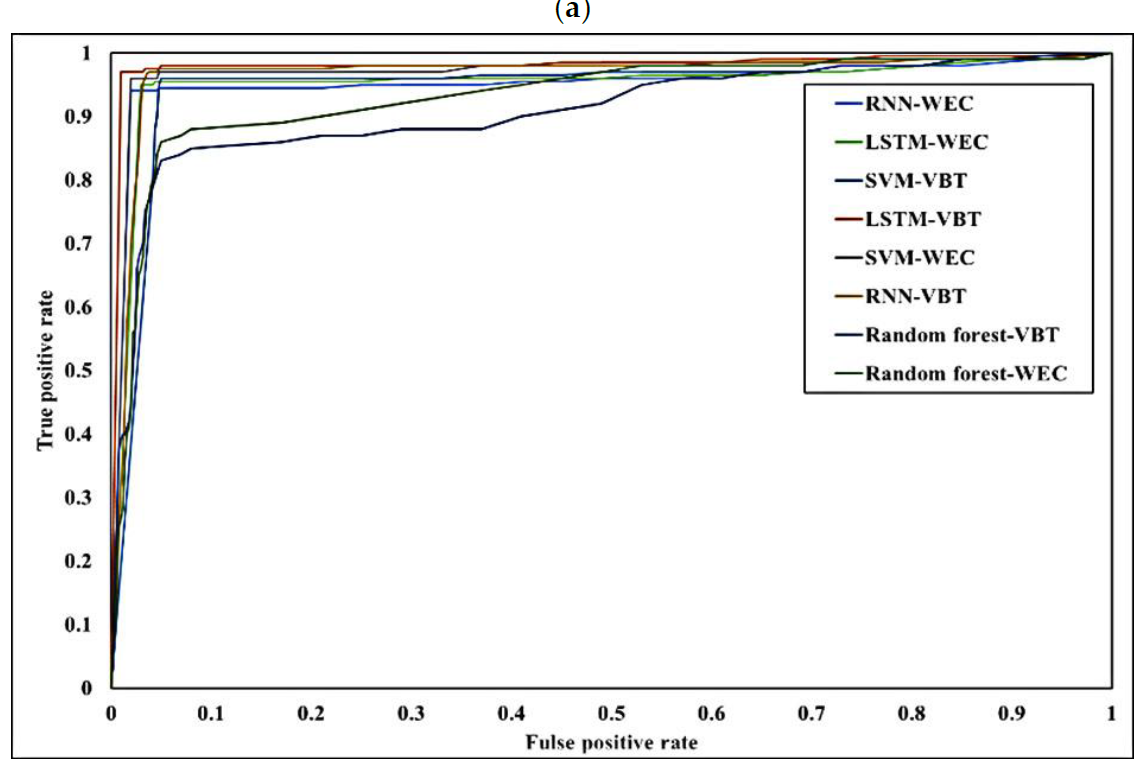
\includegraphics[height=3in]{figures/Mahsa_res3.PNG}
\caption{Figura 5-a de \cite{Mahsa}: Curvas ROC de los modelos.}
\label{Mahsa_res3}
\end{figure}

% \begin{figure}[h!]
% \centering
% 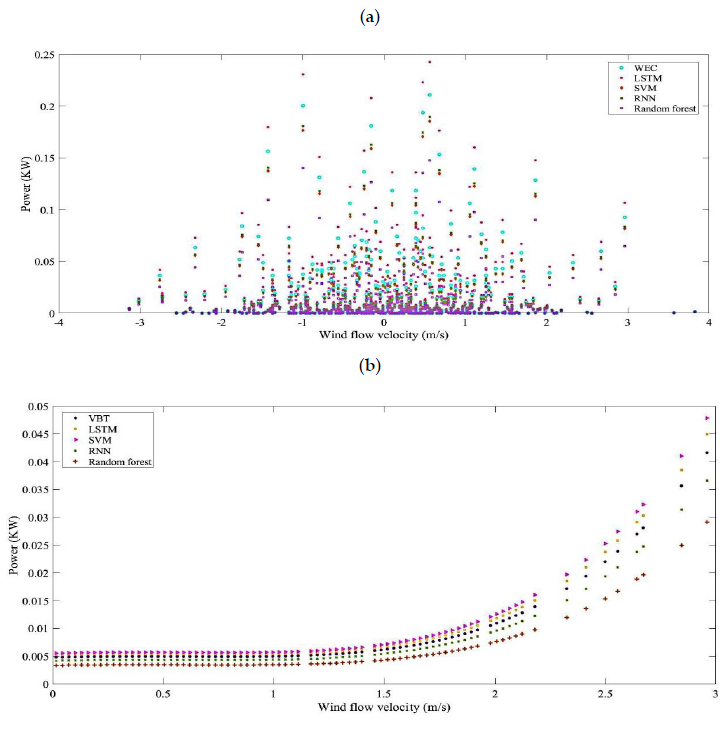
\includegraphics[height=5in]{figures/Mahsa_res2.PNG}
% \caption{Figura 4 de \cite{Mahsa}: potencia simulada para (a) VBT y (b) Searaser.}
% \label{Mahsa_res2}
% \end{figure}


\section{Conclusiones}

\begin{table}
\centering
% \begin{turn}{90}
\begin{tabular}{|l l l|}
\hline
Modelo  & Hiperparámetros & cita\\
\hline
    &&\\
RF  &&\\
    &  $N_{est}= 1-200$ , $min_{samp-leaf} =  1-5$& \\

KNN &&\\
    & $n_{neigh}= 1-50$ &\\
    &p$esos = uniforme, distancia$&\\
 

NN  &&\\
    &$solver = lbfgs, sgd, adam$&\\
    &$alpha = 0.0001-1000$&\\
    &$capas ocultas = 1,2,3$& \citeauthor{Manuel}\\
    &$neuronas / c. ocultas = 2-10$ (Cl), $2-20$ (Reg)&\\
    &$activación = identidad, logística, tanh, relu$&\\
    &$max_{iter} = 2000$&\\


 SVM   &&\\
     &$C = 0.1-5$ (Cl), $25-300$ (Reg)&\\
     &$kernel = rbf$&\\
     &$\gamma= 0.005-0.05$  (Cl), $0.01-0.1$ (Reg)&\\
     &$\epsilon=  0.001-20 $  (Reg)&\\


WT   &&\\
    &$clusters = 4-144$&\\
     &&\\
\hline
   &&\\
NN-BF   &&\\
    &$retardo =  1-8$,  $ capas~ocultas = 4$&\\
     &$solver = Levenberg~Marquardt$&\\
     &$learning~rate = 0.025-0.5$&\\

NN-RBF     &&\\
    &$retardo = 1-8$, $capas ocultas = 1$&\citeauthor{Li2}\\
     &$solver = Levenberg~Marquardt$&\\
     &$dispersión = 0.5-1.0$&\\
NN-ADALINE     &&\\
    &$retardo = 1-8$,$ nº capas ocultas = 4$&\\
     &$solver = LMS$&\\
     &$learning rate =$ --&\\
     &&\\
\hline
   &&\\
RNN    &&\\
        &$capas ocultas = 10$, $capas densas = 1$&\\
        &$activación = Adam$&\\
        &$epoch = 100$, $batch = 20$&\\
LSTM      &&\\
    & $iguales a RNN$&\citeauthor{Mahsa}\\
SVM-2     & -- &\\
RF-2     & -- &\\
\hline
\end{tabular}
% \end{turn}
\caption{Hiperparámetros.}
 \label{tabla}
\end{table}



\begin{table}[h!]
\centering
% \begin{turn}{90}
\begin{tabular}{|p{2.0cm}|p{7.5cm}|p{7.0cm}| }
\hline
Modelo  & Pros& Cons \\
\hline
LR (reg. logística) &- Modelo simple, 2º mejor precisión para cantidad de lluvia, simula meses con cantidad inusual de días húmedos (+ de 20)&\\
&&\\
GLM & - Modelo simple, simulan días con intensidades > 100 mm  &  - Baja precisión para int. de lluvia\\
 &&\\
RF &  - 2º mejor precisión para int.de lluvia& - Variabilidad de hiperparámetros, baja precisión para cantidad de lluvia\\
 &&\\
 KNN& -2º mejor precisión para int. de lluvia& - Variabilidad de hiperparámetros,  baja precision para cantidad de lluvia\\
 &&\\
NN& - Mejor precisión para int. de lluvia. Simula meses con + de 20 días húmedos, simula prob. de transición entre dos días húmedos& - Gran variabilidad de hiperparámetros, baja precisión para días con intensidad > 20 mm \\
&&\\
SVM   &- Simula meses con + de 20 días húmedos, 2º mejor precisión para cantidad de lluvia  &\\
 &&\\
  WT & - Preserva la correlación observada.
& - Peor precisión, fallan en meses húmedos \\
\hline
BF&Modelo más simple  &- Mínimos locales, convergencia lenta, gran variabilidad de hiperparámetros\\
&&\\
RBF&- Convergencia rápida& Gran variabilidad de hiperparámetros\\
&&\\
ADALINE&- Convergencia rápida&- Gran variabilidad de hiperparámetros\\
&&\\
\hline
RNN&- 2º mejor precision&- Desvanecimiento del gradiente,  gran variabilidad de hiperparametros\\
&&\\
LSTM&- Mejor precisión, soluciona el desvanecimiento del gradiente&- Gran variabilidad de hiperparámetros\\
&&\\
SVM-2&- Modelo más simple, precisión razonablemente buena& Variabilidad de hiperparámetros\\
RF-2&&- Baja precisión, variabilidad de hiperparámetros\\
\hline
\end{tabular}
% \end{turn}
\caption{Comparación de los modelos.}
 \label{tabla_res}
\end{table}


Se han analizado tres artículos distintos que emplean modelos de aprendizaje automático para predecir diversas magnitudes físicas en diferentes escalas temporales 
que pueden aplicarse en la puesta en marcha de dispositivos de generación de energías renovables. En la tabla \ref{tabla}  se muestra un resumen de los modelos junto con los hiperparámetros considerados y en la tabla \ref{tabla_res} un resumen de las conclusiones obtenidas para cada uno de ellos.

En el primer artículo \citep{Manuel}, se comparó el rendimiento de 8 métodos de aprendizaje automático y 
estadísticos para predecir la lluvia a largo plazo. Los métodos utilizaron patrones 
sinópticos atmosféricos para diferentes variables climáticas y espaciales como predictores en 
17 sitios localizados  en la isla de Tenerife, España. Los resultados
 muestran que la mayoría de los métodos de aprendizaje automático son muy sensibles 
a los hiperparámetros elegidos y que la selección incorrecta de estos parámetros
 puede llevar a modelos sin capacidad predictiva o que sobre-ajustan los
 datos de entrenamiento. Los resultados también indican que las redes neuronales son el mejor método 
para predecir la ocurrencia de lluvia, seguido de cerca por regresiones lineales y SVM. En cuanto a la predicción de la intensidad 
de lluvia, el rendimiento de las redes neuronales es superior al de los otros métodos. 
Por otro lado, el estudio sugiere la importancia de determinar los hiperparámetros 
óptimos para cada estación de medición de lluvia y de considerar modelos espacio-temporales 
en futuros trabajos.

En el segundo artículo, \citep{Li2}, se evaluaron diferentes modelos de redes neuronales  
para predecir la velocidad media del viento a corto plazo, es decir predicciones de una hora. Los resultados demostraron 
que la precisión de las redes neuronales en la predicción de la velocidad del viento depende fuertemente de
la estructura de las redes y de las tasas de aprendizaje.
Por lo tanto, estos parámetros se deben escoger tras realizar una búsqueda exhaustiva de hiper parámetros. 
También se encontró que el modelo óptimo para  un sitio específico puede no ser adecuado para otro sitio y 
se recomienda no utilizar un solo tipo de modelo NN para la predicción de la velocidad del viento en diferentes sitios. Por último, 
el estudio sugiere el uso de métodos de combinación de pronósticos, como el método de promedio de modelos 
bayesianos, para producir una única predicción a partir de múltiples pronósticos plausibles.

El tercer artículo, \citep{Mahsa}, se enfoca en encontrar el mejor algoritmo de ML para predecir la cantidad de energía producida por sistemas de energía renovable. Se compararon cuatro algoritmos de ML: LSTM, SVM, RNN y RF.
Se evaluaron los parámetros clave utilizados en el análisis del sistema, incluyendo la fuerza ejercida en cada dispositivo y su producción de energía. Se encontró que LSTM y RNN son los algoritmos más confiables y precisos en términos de predicción. Se utilizó una curva ROC para evaluar la precisión de los algoritmos y se encontró que LSTM fue el más preciso, por lo tanto se concluyó que el algoritmo LSTM es el más adecuado para predecir la producción de energía de sistemas de energía renovable.

Los tres artículos presentan la importancia de seleccionar los hiperparámetros óptimos para los modelos de aprendizaje automático y estadísticos en la predicción de diferentes variables climáticas. El artículo 1 y el artículo 2 hacen hincapié en la importancia de la selección adecuada de las entradas y tasas de aprendizaje para lograr una mayor precisión en la predicción de lluvia y velocidad del viento, respectivamente. Ambos artículos destacan que el modelo óptimo puede variar según la ubicación geográfica y que no se debe utilizar solo un tipo de modelo de aprendizaje automático para la predicción de diferentes variables climáticas.

Por otro lado, el artículo 3 presenta un enfoque diferente en la aplicación de modelos de aprendizaje automático en la predicción de la energía producida por diferentes sistemas híbridos. Este estudio utiliza simulaciones numéricas para medir la fuerza ejercida y la energía producida por diferentes sistemas y compara los resultados para seleccionar el más adecuado según las condiciones climáticas de la región seleccionada. Además, este estudio presenta una limitación notable debido a la incertidumbre de los resultados de un sistema específico.

En general, los tres artículos destacan la importancia de la selección adecuada de los hiperparámetros y la consideración de factores específicos de la ubicación en la aplicación de modelos de aprendizaje automático y estadísticos en la predicción de diferentes variables climáticas.



    \bibliographystyle{apalike}
    \bibliography{references}
	
\end{document}
